\documentclass{report}

%%%%%%%%%%%%%%%%%%%%%%%%%%%%%%%%%
% PACKAGE IMPORTS
%%%%%%%%%%%%%%%%%%%%%%%%%%%%%%%%%


\usepackage[tmargin=2cm,rmargin=1in,lmargin=1in,margin=0.85in,bmargin=2cm,footskip=.2in]{geometry}
\usepackage{amsmath,amsfonts,amsthm,amssymb,mathtools}
\usepackage[varbb]{newpxmath}
\usepackage{xfrac}
\usepackage[makeroom]{cancel}
\usepackage{mathtools}
\usepackage{bookmark}
\usepackage{enumitem}
\usepackage{hyperref,theoremref}
\hypersetup{
	pdftitle={Assignment},
	colorlinks=true, linkcolor=doc!90,
	bookmarksnumbered=true,
	bookmarksopen=true
}
\usepackage[most,many,breakable]{tcolorbox}
\usepackage{xcolor}
\usepackage{varwidth}
\usepackage{varwidth}
\usepackage{etoolbox}
%\usepackage{authblk}
\usepackage{nameref}
\usepackage{multicol,array}
\usepackage{tikz-cd}
\usepackage[ruled,vlined,linesnumbered]{algorithm2e}
\usepackage{comment} % enables the use of multi-line comments (\ifx \fi) 
\usepackage{import}
\usepackage{xifthen}
\usepackage{pdfpages}
\usepackage{transparent}

\newcommand\mycommfont[1]{\footnotesize\ttfamily\textcolor{blue}{#1}}
\SetCommentSty{mycommfont}
\newcommand{\incfig}[1]{%
    \def\svgwidth{\columnwidth}
    \import{./figures/}{#1.pdf_tex}
}

\usepackage{tikzsymbols}
\renewcommand\qedsymbol{$\Laughey$}


%\usepackage{import}
%\usepackage{xifthen}
%\usepackage{pdfpages}
%\usepackage{transparent}


%%%%%%%%%%%%%%%%%%%%%%%%%%%%%%
% SELF MADE COLORS
%%%%%%%%%%%%%%%%%%%%%%%%%%%%%%



\definecolor{myg}{RGB}{56, 140, 70}
\definecolor{myb}{RGB}{45, 111, 177}
\definecolor{myr}{RGB}{199, 68, 64}
\definecolor{mytheorembg}{HTML}{F2F2F9}
\definecolor{mytheoremfr}{HTML}{00007B}
\definecolor{mylenmabg}{HTML}{FFFAF8}
\definecolor{mylenmafr}{HTML}{983b0f}
\definecolor{mypropbg}{HTML}{f2fbfc}
\definecolor{mypropfr}{HTML}{191971}
\definecolor{myexamplebg}{HTML}{F2FBF8}
\definecolor{myexamplefr}{HTML}{88D6D1}
\definecolor{myexampleti}{HTML}{2A7F7F}
\definecolor{mydefinitbg}{HTML}{E5E5FF}
\definecolor{mydefinitfr}{HTML}{3F3FA3}
\definecolor{notesgreen}{RGB}{0,162,0}
\definecolor{myp}{RGB}{197, 92, 212}
\definecolor{mygr}{HTML}{2C3338}
\definecolor{myred}{RGB}{127,0,0}
\definecolor{myyellow}{RGB}{169,121,69}
\definecolor{myexercisebg}{HTML}{F2FBF8}
\definecolor{myexercisefg}{HTML}{88D6D1}


%%%%%%%%%%%%%%%%%%%%%%%%%%%%
% TCOLORBOX SETUPS
%%%%%%%%%%%%%%%%%%%%%%%%%%%%

\setlength{\parindent}{1cm}
%================================
% THEOREM BOX
%================================

\tcbuselibrary{theorems,skins,hooks}
\newtcbtheorem[number within=section]{Theorem}{Theorem}
{%
	enhanced,
	breakable,
	colback = mytheorembg,
	frame hidden,
	boxrule = 0sp,
	borderline west = {2pt}{0pt}{mytheoremfr},
	sharp corners,
	detach title,
	before upper = \tcbtitle\par\smallskip,
	coltitle = mytheoremfr,
	fonttitle = \bfseries\sffamily,
	description font = \mdseries,
	separator sign none,
	segmentation style={solid, mytheoremfr},
}
{th}

\tcbuselibrary{theorems,skins,hooks}
\newtcbtheorem[number within=chapter]{theorem}{Theorem}
{%
	enhanced,
	breakable,
	colback = mytheorembg,
	frame hidden,
	boxrule = 0sp,
	borderline west = {2pt}{0pt}{mytheoremfr},
	sharp corners,
	detach title,
	before upper = \tcbtitle\par\smallskip,
	coltitle = mytheoremfr,
	fonttitle = \bfseries\sffamily,
	description font = \mdseries,
	separator sign none,
	segmentation style={solid, mytheoremfr},
}
{th}


\tcbuselibrary{theorems,skins,hooks}
\newtcolorbox{Theoremcon}
{%
	enhanced
	,breakable
	,colback = mytheorembg
	,frame hidden
	,boxrule = 0sp
	,borderline west = {2pt}{0pt}{mytheoremfr}
	,sharp corners
	,description font = \mdseries
	,separator sign none
}

%================================
% Corollary
%================================
\tcbuselibrary{theorems,skins,hooks}
\newtcbtheorem[number within=section]{Corollary}{Corollary}
{%
	enhanced
	,breakable
	,colback = myp!10
	,frame hidden
	,boxrule = 0sp
	,borderline west = {2pt}{0pt}{myp!85!black}
	,sharp corners
	,detach title
	,before upper = \tcbtitle\par\smallskip
	,coltitle = myp!85!black
	,fonttitle = \bfseries\sffamily
	,description font = \mdseries
	,separator sign none
	,segmentation style={solid, myp!85!black}
}
{th}
\tcbuselibrary{theorems,skins,hooks}
\newtcbtheorem[number within=chapter]{corollary}{Corollary}
{%
	enhanced
	,breakable
	,colback = myp!10
	,frame hidden
	,boxrule = 0sp
	,borderline west = {2pt}{0pt}{myp!85!black}
	,sharp corners
	,detach title
	,before upper = \tcbtitle\par\smallskip
	,coltitle = myp!85!black
	,fonttitle = \bfseries\sffamily
	,description font = \mdseries
	,separator sign none
	,segmentation style={solid, myp!85!black}
}
{th}


%================================
% LENMA
%================================

\tcbuselibrary{theorems,skins,hooks}
\newtcbtheorem[number within=section]{Lenma}{Lenma}
{%
	enhanced,
	breakable,
	colback = mylenmabg,
	frame hidden,
	boxrule = 0sp,
	borderline west = {2pt}{0pt}{mylenmafr},
	sharp corners,
	detach title,
	before upper = \tcbtitle\par\smallskip,
	coltitle = mylenmafr,
	fonttitle = \bfseries\sffamily,
	description font = \mdseries,
	separator sign none,
	segmentation style={solid, mylenmafr},
}
{th}

\tcbuselibrary{theorems,skins,hooks}
\newtcbtheorem[number within=chapter]{lenma}{Lenma}
{%
	enhanced,
	breakable,
	colback = mylenmabg,
	frame hidden,
	boxrule = 0sp,
	borderline west = {2pt}{0pt}{mylenmafr},
	sharp corners,
	detach title,
	before upper = \tcbtitle\par\smallskip,
	coltitle = mylenmafr,
	fonttitle = \bfseries\sffamily,
	description font = \mdseries,
	separator sign none,
	segmentation style={solid, mylenmafr},
}
{th}


%================================
% PROPOSITION
%================================

\tcbuselibrary{theorems,skins,hooks}
\newtcbtheorem[number within=section]{Prop}{Proposition}
{%
	enhanced,
	breakable,
	colback = mypropbg,
	frame hidden,
	boxrule = 0sp,
	borderline west = {2pt}{0pt}{mypropfr},
	sharp corners,
	detach title,
	before upper = \tcbtitle\par\smallskip,
	coltitle = mypropfr,
	fonttitle = \bfseries\sffamily,
	description font = \mdseries,
	separator sign none,
	segmentation style={solid, mypropfr},
}
{th}

\tcbuselibrary{theorems,skins,hooks}
\newtcbtheorem[number within=chapter]{prop}{Proposition}
{%
	enhanced,
	breakable,
	colback = mypropbg,
	frame hidden,
	boxrule = 0sp,
	borderline west = {2pt}{0pt}{mypropfr},
	sharp corners,
	detach title,
	before upper = \tcbtitle\par\smallskip,
	coltitle = mypropfr,
	fonttitle = \bfseries\sffamily,
	description font = \mdseries,
	separator sign none,
	segmentation style={solid, mypropfr},
}
{th}


%================================
% CLAIM
%================================

\tcbuselibrary{theorems,skins,hooks}
\newtcbtheorem[number within=section]{claim}{Claim}
{%
	enhanced
	,breakable
	,colback = myg!10
	,frame hidden
	,boxrule = 0sp
	,borderline west = {2pt}{0pt}{myg}
	,sharp corners
	,detach title
	,before upper = \tcbtitle\par\smallskip
	,coltitle = myg!85!black
	,fonttitle = \bfseries\sffamily
	,description font = \mdseries
	,separator sign none
	,segmentation style={solid, myg!85!black}
}
{th}



%================================
% Exercise
%================================

\tcbuselibrary{theorems,skins,hooks}
\newtcbtheorem[number within=section]{Exercise}{Exercise}
{%
	enhanced,
	breakable,
	colback = myexercisebg,
	frame hidden,
	boxrule = 0sp,
	borderline west = {2pt}{0pt}{myexercisefg},
	sharp corners,
	detach title,
	before upper = \tcbtitle\par\smallskip,
	coltitle = myexercisefg,
	fonttitle = \bfseries\sffamily,
	description font = \mdseries,
	separator sign none,
	segmentation style={solid, myexercisefg},
}
{th}

\tcbuselibrary{theorems,skins,hooks}
\newtcbtheorem[number within=chapter]{exercise}{Exercise}
{%
	enhanced,
	breakable,
	colback = myexercisebg,
	frame hidden,
	boxrule = 0sp,
	borderline west = {2pt}{0pt}{myexercisefg},
	sharp corners,
	detach title,
	before upper = \tcbtitle\par\smallskip,
	coltitle = myexercisefg,
	fonttitle = \bfseries\sffamily,
	description font = \mdseries,
	separator sign none,
	segmentation style={solid, myexercisefg},
}
{th}

%================================
% EXAMPLE BOX
%================================

\newtcbtheorem[number within=section]{Example}{Example}
{%
	colback = myexamplebg
	,breakable
	,colframe = myexamplefr
	,coltitle = myexampleti
	,boxrule = 1pt
	,sharp corners
	,detach title
	,before upper=\tcbtitle\par\smallskip
	,fonttitle = \bfseries
	,description font = \mdseries
	,separator sign none
	,description delimiters parenthesis
}
{ex}

\newtcbtheorem[number within=chapter]{example}{Example}
{%
	colback = myexamplebg
	,breakable
	,colframe = myexamplefr
	,coltitle = myexampleti
	,boxrule = 1pt
	,sharp corners
	,detach title
	,before upper=\tcbtitle\par\smallskip
	,fonttitle = \bfseries
	,description font = \mdseries
	,separator sign none
	,description delimiters parenthesis
}
{ex}

%================================
% DEFINITION BOX
%================================

\newtcbtheorem[number within=section]{Definition}{Definition}{enhanced,
	before skip=2mm,after skip=2mm, colback=red!5,colframe=red!80!black,boxrule=0.5mm,
	attach boxed title to top left={xshift=1cm,yshift*=1mm-\tcboxedtitleheight}, varwidth boxed title*=-3cm,
	boxed title style={frame code={
					\path[fill=tcbcolback]
					([yshift=-1mm,xshift=-1mm]frame.north west)
					arc[start angle=0,end angle=180,radius=1mm]
					([yshift=-1mm,xshift=1mm]frame.north east)
					arc[start angle=180,end angle=0,radius=1mm];
					\path[left color=tcbcolback!60!black,right color=tcbcolback!60!black,
						middle color=tcbcolback!80!black]
					([xshift=-2mm]frame.north west) -- ([xshift=2mm]frame.north east)
					[rounded corners=1mm]-- ([xshift=1mm,yshift=-1mm]frame.north east)
					-- (frame.south east) -- (frame.south west)
					-- ([xshift=-1mm,yshift=-1mm]frame.north west)
					[sharp corners]-- cycle;
				},interior engine=empty,
		},
	fonttitle=\bfseries,
	title={#2},#1}{def}
\newtcbtheorem[number within=chapter]{definition}{Definition}{enhanced,
	before skip=2mm,after skip=2mm, colback=red!5,colframe=red!80!black,boxrule=0.5mm,
	attach boxed title to top left={xshift=1cm,yshift*=1mm-\tcboxedtitleheight}, varwidth boxed title*=-3cm,
	boxed title style={frame code={
					\path[fill=tcbcolback]
					([yshift=-1mm,xshift=-1mm]frame.north west)
					arc[start angle=0,end angle=180,radius=1mm]
					([yshift=-1mm,xshift=1mm]frame.north east)
					arc[start angle=180,end angle=0,radius=1mm];
					\path[left color=tcbcolback!60!black,right color=tcbcolback!60!black,
						middle color=tcbcolback!80!black]
					([xshift=-2mm]frame.north west) -- ([xshift=2mm]frame.north east)
					[rounded corners=1mm]-- ([xshift=1mm,yshift=-1mm]frame.north east)
					-- (frame.south east) -- (frame.south west)
					-- ([xshift=-1mm,yshift=-1mm]frame.north west)
					[sharp corners]-- cycle;
				},interior engine=empty,
		},
	fonttitle=\bfseries,
	title={#2},#1}{def}



%================================
% Solution BOX
%================================

\makeatletter
\newtcbtheorem{question}{Question}{enhanced,
	breakable,
	colback=white,
	colframe=myb!80!black,
	attach boxed title to top left={yshift*=-\tcboxedtitleheight},
	fonttitle=\bfseries,
	title={#2},
	boxed title size=title,
	boxed title style={%
			sharp corners,
			rounded corners=northwest,
			colback=tcbcolframe,
			boxrule=0pt,
		},
	underlay boxed title={%
			\path[fill=tcbcolframe] (title.south west)--(title.south east)
			to[out=0, in=180] ([xshift=5mm]title.east)--
			(title.center-|frame.east)
			[rounded corners=\kvtcb@arc] |-
			(frame.north) -| cycle;
		},
	#1
}{def}
\makeatother

%================================
% SOLUTION BOX
%================================

\makeatletter
\newtcolorbox{solution}{enhanced,
	breakable,
	colback=white,
	colframe=myg!80!black,
	attach boxed title to top left={yshift*=-\tcboxedtitleheight},
	title=Solution,
	boxed title size=title,
	boxed title style={%
			sharp corners,
			rounded corners=northwest,
			colback=tcbcolframe,
			boxrule=0pt,
		},
	underlay boxed title={%
			\path[fill=tcbcolframe] (title.south west)--(title.south east)
			to[out=0, in=180] ([xshift=5mm]title.east)--
			(title.center-|frame.east)
			[rounded corners=\kvtcb@arc] |-
			(frame.north) -| cycle;
		},
}
\makeatother

%================================
% Question BOX
%================================

\makeatletter
\newtcbtheorem{qstion}{Question}{enhanced,
	breakable,
	colback=white,
	colframe=mygr,
	attach boxed title to top left={yshift*=-\tcboxedtitleheight},
	fonttitle=\bfseries,
	title={#2},
	boxed title size=title,
	boxed title style={%
			sharp corners,
			rounded corners=northwest,
			colback=tcbcolframe,
			boxrule=0pt,
		},
	underlay boxed title={%
			\path[fill=tcbcolframe] (title.south west)--(title.south east)
			to[out=0, in=180] ([xshift=5mm]title.east)--
			(title.center-|frame.east)
			[rounded corners=\kvtcb@arc] |-
			(frame.north) -| cycle;
		},
	#1
}{def}
\makeatother

\newtcbtheorem[number within=chapter]{wconc}{Wrong Concept}{
	breakable,
	enhanced,
	colback=white,
	colframe=myr,
	arc=0pt,
	outer arc=0pt,
	fonttitle=\bfseries\sffamily\large,
	colbacktitle=myr,
	attach boxed title to top left={},
	boxed title style={
			enhanced,
			skin=enhancedfirst jigsaw,
			arc=3pt,
			bottom=0pt,
			interior style={fill=myr}
		},
	#1
}{def}



%================================
% NOTE BOX
%================================

\usetikzlibrary{arrows,calc,shadows.blur}
\tcbuselibrary{skins}
\newtcolorbox{note}[1][]{%
	enhanced jigsaw,
	colback=gray!20!white,%
	colframe=gray!80!black,
	size=small,
	boxrule=1pt,
	title=\textbf{Note:-},
	halign title=flush center,
	coltitle=black,
	breakable,
	drop shadow=black!50!white,
	attach boxed title to top left={xshift=1cm,yshift=-\tcboxedtitleheight/2,yshifttext=-\tcboxedtitleheight/2},
	minipage boxed title=1.5cm,
	boxed title style={%
			colback=white,
			size=fbox,
			boxrule=1pt,
			boxsep=2pt,
			underlay={%
					\coordinate (dotA) at ($(interior.west) + (-0.5pt,0)$);
					\coordinate (dotB) at ($(interior.east) + (0.5pt,0)$);
					\begin{scope}
						\clip (interior.north west) rectangle ([xshift=3ex]interior.east);
						\filldraw [white, blur shadow={shadow opacity=60, shadow yshift=-.75ex}, rounded corners=2pt] (interior.north west) rectangle (interior.south east);
					\end{scope}
					\begin{scope}[gray!80!black]
						\fill (dotA) circle (2pt);
						\fill (dotB) circle (2pt);
					\end{scope}
				},
		},
	#1,
}

%%%%%%%%%%%%%%%%%%%%%%%%%%%%%%
% SELF MADE COMMANDS
%%%%%%%%%%%%%%%%%%%%%%%%%%%%%%


\newcommand{\thm}[2]{\begin{Theorem}{#1}{}#2\end{Theorem}}
\newcommand{\cor}[2]{\begin{Corollary}{#1}{}#2\end{Corollary}}
\newcommand{\mlenma}[2]{\begin{Lenma}{#1}{}#2\end{Lenma}}
\newcommand{\mprop}[2]{\begin{Prop}{#1}{}#2\end{Prop}}
\newcommand{\clm}[3]{\begin{claim}{#1}{#2}#3\end{claim}}
\newcommand{\wc}[2]{\begin{wconc}{#1}{}\setlength{\parindent}{1cm}#2\end{wconc}}
\newcommand{\thmcon}[1]{\begin{Theoremcon}{#1}\end{Theoremcon}}
\newcommand{\ex}[2]{\begin{Example}{#1}{}#2\end{Example}}
\newcommand{\dfn}[2]{\begin{Definition}[colbacktitle=red!75!black]{#1}{}#2\end{Definition}}
\newcommand{\dfnc}[2]{\begin{definition}[colbacktitle=red!75!black]{#1}{}#2\end{definition}}
\newcommand{\qs}[2]{\begin{question}{#1}{}#2\end{question}}
\newcommand{\pf}[2]{\begin{myproof}[#1]#2\end{myproof}}
\newcommand{\nt}[1]{\begin{note}#1\end{note}}

\newcommand*\circled[1]{\tikz[baseline=(char.base)]{
		\node[shape=circle,draw,inner sep=1pt] (char) {#1};}}
\newcommand\getcurrentref[1]{%
	\ifnumequal{\value{#1}}{0}
	{??}
	{\the\value{#1}}%
}
\newcommand{\getCurrentSectionNumber}{\getcurrentref{section}}
\newenvironment{myproof}[1][\proofname]{%
	\proof[\bfseries #1: ]%
}{\endproof}

\newcommand{\mclm}[2]{\begin{myclaim}[#1]#2\end{myclaim}}
\newenvironment{myclaim}[1][\claimname]{\proof[\bfseries #1: ]}{}

\newcounter{mylabelcounter}

\makeatletter
\newcommand{\setword}[2]{%
	\phantomsection
	#1\def\@currentlabel{\unexpanded{#1}}\label{#2}%
}
\makeatother




\tikzset{
	symbol/.style={
			draw=none,
			every to/.append style={
					edge node={node [sloped, allow upside down, auto=false]{$#1$}}}
		}
}


% deliminators
\DeclarePairedDelimiter{\abs}{\lvert}{\rvert}
\DeclarePairedDelimiter{\norm}{\lVert}{\rVert}

\DeclarePairedDelimiter{\ceil}{\lceil}{\rceil}
\DeclarePairedDelimiter{\floor}{\lfloor}{\rfloor}
\DeclarePairedDelimiter{\round}{\lfloor}{\rceil}

\newsavebox\diffdbox
\newcommand{\slantedromand}{{\mathpalette\makesl{d}}}
\newcommand{\makesl}[2]{%
\begingroup
\sbox{\diffdbox}{$\mathsurround=0pt#1\mathrm{#2}$}%
\pdfsave
\pdfsetmatrix{1 0 0.2 1}%
\rlap{\usebox{\diffdbox}}%
\pdfrestore
\hskip\wd\diffdbox
\endgroup
}
\newcommand{\dd}[1][]{\ensuremath{\mathop{}\!\ifstrempty{#1}{%
\slantedromand\@ifnextchar^{\hspace{0.2ex}}{\hspace{0.1ex}}}%
{\slantedromand\hspace{0.2ex}^{#1}}}}
\ProvideDocumentCommand\dv{o m g}{%
  \ensuremath{%
    \IfValueTF{#3}{%
      \IfNoValueTF{#1}{%
        \frac{\dd #2}{\dd #3}%
      }{%
        \frac{\dd^{#1} #2}{\dd #3^{#1}}%
      }%
    }{%
      \IfNoValueTF{#1}{%
        \frac{\dd}{\dd #2}%
      }{%
        \frac{\dd^{#1}}{\dd #2^{#1}}%
      }%
    }%
  }%
}
\providecommand*{\pdv}[3][]{\frac{\partial^{#1}#2}{\partial#3^{#1}}}
%  - others
\DeclareMathOperator{\Lap}{\mathcal{L}}
\DeclareMathOperator{\Var}{Var} % varience
\DeclareMathOperator{\Cov}{Cov} % covarience
\DeclareMathOperator{\E}{E} % expected

% Since the amsthm package isn't loaded

% I prefer the slanted \leq
\let\oldleq\leq % save them in case they're every wanted
\let\oldgeq\geq
\renewcommand{\leq}{\leqslant}
\renewcommand{\geq}{\geqslant}

% % redefine matrix env to allow for alignment, use r as default
% \renewcommand*\env@matrix[1][r]{\hskip -\arraycolsep
%     \let\@ifnextchar\new@ifnextchar
%     \array{*\c@MaxMatrixCols #1}}


%\usepackage{framed}
%\usepackage{titletoc}
%\usepackage{etoolbox}
%\usepackage{lmodern}


%\patchcmd{\tableofcontents}{\contentsname}{\sffamily\contentsname}{}{}

%\renewenvironment{leftbar}
%{\def\FrameCommand{\hspace{6em}%
%		{\color{myyellow}\vrule width 2pt depth 6pt}\hspace{1em}}%
%	\MakeFramed{\parshape 1 0cm \dimexpr\textwidth-6em\relax\FrameRestore}\vskip2pt%
%}
%{\endMakeFramed}

%\titlecontents{chapter}
%[0em]{\vspace*{2\baselineskip}}
%{\parbox{4.5em}{%
%		\hfill\Huge\sffamily\bfseries\color{myred}\thecontentspage}%
%	\vspace*{-2.3\baselineskip}\leftbar\textsc{\small\chaptername~\thecontentslabel}\\\sffamily}
%{}{\endleftbar}
%\titlecontents{section}
%[8.4em]
%{\sffamily\contentslabel{3em}}{}{}
%{\hspace{0.5em}\nobreak\itshape\color{myred}\contentspage}
%\titlecontents{subsection}
%[8.4em]
%{\sffamily\contentslabel{3em}}{}{}  
%{\hspace{0.5em}\nobreak\itshape\color{myred}\contentspage}



%%%%%%%%%%%%%%%%%%%%%%%%%%%%%%%%%%%%%%%%%%%
% TABLE OF CONTENTS
%%%%%%%%%%%%%%%%%%%%%%%%%%%%%%%%%%%%%%%%%%%

\usepackage{tikz}
\definecolor{doc}{RGB}{0,60,110}
\usepackage{titletoc}
\contentsmargin{0cm}
\titlecontents{chapter}[3.7pc]
{\addvspace{30pt}%
	\begin{tikzpicture}[remember picture, overlay]%
		\draw[fill=doc!60,draw=doc!60] (-7,-.1) rectangle (-0.9,.5);%
		\pgftext[left,x=-3.5cm,y=0.2cm]{\color{white}\Large\sc\bfseries Chapter\ \thecontentslabel};%
	\end{tikzpicture}\color{doc!60}\large\sc\bfseries}%
{}
{}
{\;\titlerule\;\large\sc\bfseries Page \thecontentspage
	\begin{tikzpicture}[remember picture, overlay]
		\draw[fill=doc!60,draw=doc!60] (2pt,0) rectangle (4,0.1pt);
	\end{tikzpicture}}%
\titlecontents{section}[3.7pc]
{\addvspace{2pt}}
{\contentslabel[\thecontentslabel]{2pc}}
{}
{\hfill\small \thecontentspage}
[]
\titlecontents*{subsection}[3.7pc]
{\addvspace{-1pt}\small}
{}
{}
{\ --- \small\thecontentspage}
[ \textbullet\ ][]

\makeatletter
\renewcommand{\tableofcontents}{%
	\chapter*{%
	  \vspace*{-20\p@}%
	  \begin{tikzpicture}[remember picture, overlay]%
		  \pgftext[right,x=15cm,y=0.2cm]{\color{doc!60}\Huge\sc\bfseries \contentsname};%
		  \draw[fill=doc!60,draw=doc!60] (13,-.75) rectangle (20,1);%
		  \clip (13,-.75) rectangle (20,1);
		  \pgftext[right,x=15cm,y=0.2cm]{\color{white}\Huge\sc\bfseries \contentsname};%
	  \end{tikzpicture}}%
	\@starttoc{toc}}
\makeatother

%From M275 "Topology" at SJSU
\newcommand{\id}{\mathrm{id}}
\newcommand{\taking}[1]{\xrightarrow{#1}}
\newcommand{\inv}{^{-1}}

%From M170 "Introduction to Graph Theory" at SJSU
\DeclareMathOperator{\diam}{diam}
\DeclareMathOperator{\ord}{ord}
\newcommand{\defeq}{\overset{\mathrm{def}}{=}}

%From the USAMO .tex files
\newcommand{\ts}{\textsuperscript}
\newcommand{\dg}{^\circ}
\newcommand{\ii}{\item}

% % From Math 55 and Math 145 at Harvard
% \newenvironment{subproof}[1][Proof]{%
% \begin{proof}[#1] \renewcommand{\qedsymbol}{$\blacksquare$}}%
% {\end{proof}}

\newcommand{\liff}{\leftrightarrow}
\newcommand{\lthen}{\rightarrow}
\newcommand{\opname}{\operatorname}
\newcommand{\surjto}{\twoheadrightarrow}
\newcommand{\injto}{\hookrightarrow}
\newcommand{\On}{\mathrm{On}} % ordinals
\DeclareMathOperator{\img}{im} % Image
\DeclareMathOperator{\Img}{Im} % Image
\DeclareMathOperator{\coker}{coker} % Cokernel
\DeclareMathOperator{\Coker}{Coker} % Cokernel
\DeclareMathOperator{\Ker}{Ker} % Kernel
\DeclareMathOperator{\rank}{rank}
\DeclareMathOperator{\Spec}{Spec} % spectrum
\DeclareMathOperator{\Tr}{Tr} % trace
\DeclareMathOperator{\pr}{pr} % projection
\DeclareMathOperator{\ext}{ext} % extension
\DeclareMathOperator{\pred}{pred} % predecessor
\DeclareMathOperator{\dom}{dom} % domain
\DeclareMathOperator{\ran}{ran} % range
\DeclareMathOperator{\Hom}{Hom} % homomorphism
\DeclareMathOperator{\Mor}{Mor} % morphisms
\DeclareMathOperator{\End}{End} % endomorphism

\def\shrug{\texttt{\raisebox{0.75em}{\char`\_}\char`\\\char`\_\kern-0.5ex(\kern-0.25ex\raisebox{0.25ex}{\rotatebox{45}{\raisebox{-.75ex}"\kern-1.5ex\rotatebox{-90})}}\kern-0.5ex)\kern-0.5ex\char`\_/\raisebox{0.75em}{\char`\_}}} 

\newcommand{\eps}{\epsilon}
\newcommand{\veps}{\varepsilon}
\newcommand{\ol}{\overline}
\newcommand{\ul}{\underline}
\newcommand{\wt}{\widetilde}
\newcommand{\wh}{\widehat}
\newcommand{\vocab}[1]{\textbf{\color{blue} #1}}
\providecommand{\half}{\frac{1}{2}}
\newcommand{\dang}{\measuredangle} %% Directed angle
\newcommand{\ray}[1]{\overrightarrow{#1}}
\newcommand{\seg}[1]{\overline{#1}}
\newcommand{\arc}[1]{\wideparen{#1}}
\DeclareMathOperator{\cis}{cis}
\DeclareMathOperator*{\lcm}{lcm}
\DeclareMathOperator*{\argmin}{arg min}
\DeclareMathOperator*{\argmax}{arg max}
\newcommand{\cycsum}{\sum_{\mathrm{cyc}}}
\newcommand{\symsum}{\sum_{\mathrm{sym}}}
\newcommand{\cycprod}{\prod_{\mathrm{cyc}}}
\newcommand{\symprod}{\prod_{\mathrm{sym}}}
\newcommand{\Qed}{\begin{flushright}\qed\end{flushright}}
\newcommand{\parinn}{\setlength{\parindent}{1cm}}
\newcommand{\parinf}{\setlength{\parindent}{0cm}}
% \newcommand{\norm}{\|\cdot\|}
\newcommand{\inorm}{\norm_{\infty}}
\newcommand{\opensets}{\{V_{\alpha}\}_{\alpha\in I}}
\newcommand{\oset}{V_{\alpha}}
\newcommand{\opset}[1]{V_{\alpha_{#1}}}
\newcommand{\lub}{\text{lub}}
\newcommand{\del}[2]{\frac{\partial #1}{\partial #2}}
\newcommand{\Del}[3]{\frac{\partial^{#1} #2}{\partial^{#1} #3}}
\newcommand{\deld}[2]{\dfrac{\partial #1}{\partial #2}}
\newcommand{\Deld}[3]{\dfrac{\partial^{#1} #2}{\partial^{#1} #3}}
\newcommand{\lm}{\lambda}
\newcommand{\uin}{\mathbin{\rotatebox[origin=c]{90}{$\in$}}}
\newcommand{\usubset}{\mathbin{\rotatebox[origin=c]{90}{$\subset$}}}
\newcommand{\lt}{\left}
\newcommand{\rt}{\right}
\newcommand{\bs}[1]{\boldsymbol{#1}}
\newcommand{\exs}{\exists}
\newcommand{\st}{\strut}
\newcommand{\dps}[1]{\displaystyle{#1}}

\newcommand{\sol}{\setlength{\parindent}{0cm}\textbf{\textit{Solution:}}\setlength{\parindent}{1cm} }
\newcommand{\solve}[1]{\setlength{\parindent}{0cm}\textbf{\textit{Solution: }}\setlength{\parindent}{1cm}#1 \Qed}
% Things Lie
\newcommand{\kb}{\mathfrak b}
\newcommand{\kg}{\mathfrak g}
\newcommand{\kh}{\mathfrak h}
\newcommand{\kn}{\mathfrak n}
\newcommand{\ku}{\mathfrak u}
\newcommand{\kz}{\mathfrak z}
\DeclareMathOperator{\Ext}{Ext} % Ext functor
\DeclareMathOperator{\Tor}{Tor} % Tor functor
\newcommand{\gl}{\opname{\mathfrak{gl}}} % frak gl group
\renewcommand{\sl}{\opname{\mathfrak{sl}}} % frak sl group chktex 6

% More script letters etc.
\newcommand{\SA}{\mathcal A}
\newcommand{\SB}{\mathcal B}
\newcommand{\SC}{\mathcal C}
\newcommand{\SF}{\mathcal F}
\newcommand{\SG}{\mathcal G}
\newcommand{\SH}{\mathcal H}
\newcommand{\OO}{\mathcal O}

\newcommand{\SCA}{\mathscr A}
\newcommand{\SCB}{\mathscr B}
\newcommand{\SCC}{\mathscr C}
\newcommand{\SCD}{\mathscr D}
\newcommand{\SCE}{\mathscr E}
\newcommand{\SCF}{\mathscr F}
\newcommand{\SCG}{\mathscr G}
\newcommand{\SCH}{\mathscr H}

% Mathfrak primes
\newcommand{\km}{\mathfrak m}
\newcommand{\kp}{\mathfrak p}
\newcommand{\kq}{\mathfrak q}

% number sets
\newcommand{\RR}[1][]{\ensuremath{\ifstrempty{#1}{\mathbb{R}}{\mathbb{R}^{#1}}}}
\newcommand{\NN}[1][]{\ensuremath{\ifstrempty{#1}{\mathbb{N}}{\mathbb{N}^{#1}}}}
\newcommand{\ZZ}[1][]{\ensuremath{\ifstrempty{#1}{\mathbb{Z}}{\mathbb{Z}^{#1}}}}
\newcommand{\QQ}[1][]{\ensuremath{\ifstrempty{#1}{\mathbb{Q}}{\mathbb{Q}^{#1}}}}
\newcommand{\CC}[1][]{\ensuremath{\ifstrempty{#1}{\mathbb{C}}{\mathbb{C}^{#1}}}}
\newcommand{\PP}[1][]{\ensuremath{\ifstrempty{#1}{\mathbb{P}}{\mathbb{P}^{#1}}}}
\newcommand{\HH}[1][]{\ensuremath{\ifstrempty{#1}{\mathbb{H}}{\mathbb{H}^{#1}}}}
\newcommand{\FF}[1][]{\ensuremath{\ifstrempty{#1}{\mathbb{F}}{\mathbb{F}^{#1}}}}
% expected value
\newcommand{\EE}{\ensuremath{\mathbb{E}}}
\newcommand{\charin}{\text{ char }}
\DeclareMathOperator{\sign}{sign}
\DeclareMathOperator{\Aut}{Aut}
\DeclareMathOperator{\Inn}{Inn}
\DeclareMathOperator{\Syl}{Syl}
\DeclareMathOperator{\Gal}{Gal}
\DeclareMathOperator{\GL}{GL} % General linear group
\DeclareMathOperator{\SL}{SL} % Special linear group

%---------------------------------------
% BlackBoard Math Fonts :-
%---------------------------------------

%Captital Letters
\newcommand{\bbA}{\mathbb{A}}	\newcommand{\bbB}{\mathbb{B}}
\newcommand{\bbC}{\mathbb{C}}	\newcommand{\bbD}{\mathbb{D}}
\newcommand{\bbE}{\mathbb{E}}	\newcommand{\bbF}{\mathbb{F}}
\newcommand{\bbG}{\mathbb{G}}	\newcommand{\bbH}{\mathbb{H}}
\newcommand{\bbI}{\mathbb{I}}	\newcommand{\bbJ}{\mathbb{J}}
\newcommand{\bbK}{\mathbb{K}}	\newcommand{\bbL}{\mathbb{L}}
\newcommand{\bbM}{\mathbb{M}}	\newcommand{\bbN}{\mathbb{N}}
\newcommand{\bbO}{\mathbb{O}}	\newcommand{\bbP}{\mathbb{P}}
\newcommand{\bbQ}{\mathbb{Q}}	\newcommand{\bbR}{\mathbb{R}}
\newcommand{\bbS}{\mathbb{S}}	\newcommand{\bbT}{\mathbb{T}}
\newcommand{\bbU}{\mathbb{U}}	\newcommand{\bbV}{\mathbb{V}}
\newcommand{\bbW}{\mathbb{W}}	\newcommand{\bbX}{\mathbb{X}}
\newcommand{\bbY}{\mathbb{Y}}	\newcommand{\bbZ}{\mathbb{Z}}

%---------------------------------------
% MathCal Fonts :-
%---------------------------------------

%Captital Letters
\newcommand{\mcA}{\mathcal{A}}	\newcommand{\mcB}{\mathcal{B}}
\newcommand{\mcC}{\mathcal{C}}	\newcommand{\mcD}{\mathcal{D}}
\newcommand{\mcE}{\mathcal{E}}	\newcommand{\mcF}{\mathcal{F}}
\newcommand{\mcG}{\mathcal{G}}	\newcommand{\mcH}{\mathcal{H}}
\newcommand{\mcI}{\mathcal{I}}	\newcommand{\mcJ}{\mathcal{J}}
\newcommand{\mcK}{\mathcal{K}}	\newcommand{\mcL}{\mathcal{L}}
\newcommand{\mcM}{\mathcal{M}}	\newcommand{\mcN}{\mathcal{N}}
\newcommand{\mcO}{\mathcal{O}}	\newcommand{\mcP}{\mathcal{P}}
\newcommand{\mcQ}{\mathcal{Q}}	\newcommand{\mcR}{\mathcal{R}}
\newcommand{\mcS}{\mathcal{S}}	\newcommand{\mcT}{\mathcal{T}}
\newcommand{\mcU}{\mathcal{U}}	\newcommand{\mcV}{\mathcal{V}}
\newcommand{\mcW}{\mathcal{W}}	\newcommand{\mcX}{\mathcal{X}}
\newcommand{\mcY}{\mathcal{Y}}	\newcommand{\mcZ}{\mathcal{Z}}


%---------------------------------------
% Bold Math Fonts :-
%---------------------------------------

%Captital Letters
\newcommand{\bmA}{\boldsymbol{A}}	\newcommand{\bmB}{\boldsymbol{B}}
\newcommand{\bmC}{\boldsymbol{C}}	\newcommand{\bmD}{\boldsymbol{D}}
\newcommand{\bmE}{\boldsymbol{E}}	\newcommand{\bmF}{\boldsymbol{F}}
\newcommand{\bmG}{\boldsymbol{G}}	\newcommand{\bmH}{\boldsymbol{H}}
\newcommand{\bmI}{\boldsymbol{I}}	\newcommand{\bmJ}{\boldsymbol{J}}
\newcommand{\bmK}{\boldsymbol{K}}	\newcommand{\bmL}{\boldsymbol{L}}
\newcommand{\bmM}{\boldsymbol{M}}	\newcommand{\bmN}{\boldsymbol{N}}
\newcommand{\bmO}{\boldsymbol{O}}	\newcommand{\bmP}{\boldsymbol{P}}
\newcommand{\bmQ}{\boldsymbol{Q}}	\newcommand{\bmR}{\boldsymbol{R}}
\newcommand{\bmS}{\boldsymbol{S}}	\newcommand{\bmT}{\boldsymbol{T}}
\newcommand{\bmU}{\boldsymbol{U}}	\newcommand{\bmV}{\boldsymbol{V}}
\newcommand{\bmW}{\boldsymbol{W}}	\newcommand{\bmX}{\boldsymbol{X}}
\newcommand{\bmY}{\boldsymbol{Y}}	\newcommand{\bmZ}{\boldsymbol{Z}}
%Small Letters
\newcommand{\bma}{\boldsymbol{a}}	\newcommand{\bmb}{\boldsymbol{b}}
\newcommand{\bmc}{\boldsymbol{c}}	\newcommand{\bmd}{\boldsymbol{d}}
\newcommand{\bme}{\boldsymbol{e}}	\newcommand{\bmf}{\boldsymbol{f}}
\newcommand{\bmg}{\boldsymbol{g}}	\newcommand{\bmh}{\boldsymbol{h}}
\newcommand{\bmi}{\boldsymbol{i}}	\newcommand{\bmj}{\boldsymbol{j}}
\newcommand{\bmk}{\boldsymbol{k}}	\newcommand{\bml}{\boldsymbol{l}}
\newcommand{\bmm}{\boldsymbol{m}}	\newcommand{\bmn}{\boldsymbol{n}}
\newcommand{\bmo}{\boldsymbol{o}}	\newcommand{\bmp}{\boldsymbol{p}}
\newcommand{\bmq}{\boldsymbol{q}}	\newcommand{\bmr}{\boldsymbol{r}}
\newcommand{\bms}{\boldsymbol{s}}	\newcommand{\bmt}{\boldsymbol{t}}
\newcommand{\bmu}{\boldsymbol{u}}	\newcommand{\bmv}{\boldsymbol{v}}
\newcommand{\bmw}{\boldsymbol{w}}	\newcommand{\bmx}{\boldsymbol{x}}
\newcommand{\bmy}{\boldsymbol{y}}	\newcommand{\bmz}{\boldsymbol{z}}

%---------------------------------------
% Scr Math Fonts :-
%---------------------------------------

\newcommand{\sA}{{\mathscr{A}}}   \newcommand{\sB}{{\mathscr{B}}}
\newcommand{\sC}{{\mathscr{C}}}   \newcommand{\sD}{{\mathscr{D}}}
\newcommand{\sE}{{\mathscr{E}}}   \newcommand{\sF}{{\mathscr{F}}}
\newcommand{\sG}{{\mathscr{G}}}   \newcommand{\sH}{{\mathscr{H}}}
\newcommand{\sI}{{\mathscr{I}}}   \newcommand{\sJ}{{\mathscr{J}}}
\newcommand{\sK}{{\mathscr{K}}}   \newcommand{\sL}{{\mathscr{L}}}
\newcommand{\sM}{{\mathscr{M}}}   \newcommand{\sN}{{\mathscr{N}}}
\newcommand{\sO}{{\mathscr{O}}}   \newcommand{\sP}{{\mathscr{P}}}
\newcommand{\sQ}{{\mathscr{Q}}}   \newcommand{\sR}{{\mathscr{R}}}
\newcommand{\sS}{{\mathscr{S}}}   \newcommand{\sT}{{\mathscr{T}}}
\newcommand{\sU}{{\mathscr{U}}}   \newcommand{\sV}{{\mathscr{V}}}
\newcommand{\sW}{{\mathscr{W}}}   \newcommand{\sX}{{\mathscr{X}}}
\newcommand{\sY}{{\mathscr{Y}}}   \newcommand{\sZ}{{\mathscr{Z}}}


%---------------------------------------
% Math Fraktur Font
%---------------------------------------

%Captital Letters
\newcommand{\mfA}{\mathfrak{A}}	\newcommand{\mfB}{\mathfrak{B}}
\newcommand{\mfC}{\mathfrak{C}}	\newcommand{\mfD}{\mathfrak{D}}
\newcommand{\mfE}{\mathfrak{E}}	\newcommand{\mfF}{\mathfrak{F}}
\newcommand{\mfG}{\mathfrak{G}}	\newcommand{\mfH}{\mathfrak{H}}
\newcommand{\mfI}{\mathfrak{I}}	\newcommand{\mfJ}{\mathfrak{J}}
\newcommand{\mfK}{\mathfrak{K}}	\newcommand{\mfL}{\mathfrak{L}}
\newcommand{\mfM}{\mathfrak{M}}	\newcommand{\mfN}{\mathfrak{N}}
\newcommand{\mfO}{\mathfrak{O}}	\newcommand{\mfP}{\mathfrak{P}}
\newcommand{\mfQ}{\mathfrak{Q}}	\newcommand{\mfR}{\mathfrak{R}}
\newcommand{\mfS}{\mathfrak{S}}	\newcommand{\mfT}{\mathfrak{T}}
\newcommand{\mfU}{\mathfrak{U}}	\newcommand{\mfV}{\mathfrak{V}}
\newcommand{\mfW}{\mathfrak{W}}	\newcommand{\mfX}{\mathfrak{X}}
\newcommand{\mfY}{\mathfrak{Y}}	\newcommand{\mfZ}{\mathfrak{Z}}
%Small Letters
\newcommand{\mfa}{\mathfrak{a}}	\newcommand{\mfb}{\mathfrak{b}}
\newcommand{\mfc}{\mathfrak{c}}	\newcommand{\mfd}{\mathfrak{d}}
\newcommand{\mfe}{\mathfrak{e}}	\newcommand{\mff}{\mathfrak{f}}
\newcommand{\mfg}{\mathfrak{g}}	\newcommand{\mfh}{\mathfrak{h}}
\newcommand{\mfi}{\mathfrak{i}}	\newcommand{\mfj}{\mathfrak{j}}
\newcommand{\mfk}{\mathfrak{k}}	\newcommand{\mfl}{\mathfrak{l}}
\newcommand{\mfm}{\mathfrak{m}}	\newcommand{\mfn}{\mathfrak{n}}
\newcommand{\mfo}{\mathfrak{o}}	\newcommand{\mfp}{\mathfrak{p}}
\newcommand{\mfq}{\mathfrak{q}}	\newcommand{\mfr}{\mathfrak{r}}
\newcommand{\mfs}{\mathfrak{s}}	\newcommand{\mft}{\mathfrak{t}}
\newcommand{\mfu}{\mathfrak{u}}	\newcommand{\mfv}{\mathfrak{v}}
\newcommand{\mfw}{\mathfrak{w}}	\newcommand{\mfx}{\mathfrak{x}}
\newcommand{\mfy}{\mathfrak{y}}	\newcommand{\mfz}{\mathfrak{z}}

\title{ \Huge{STA247}}
\author{Pierre's Guide}
\date{\huge{Fall 2022}}

\definecolor{titlepagecolor}{cmyk}{1,.60,0,.40}
\definecolor{namecolor}{cmyk}{1,.50,0,.10} 
\begin{document}
\begin{titlepage}

    \newgeometry{left=7.5cm} %defines the geometry for the titlepage
    \pagecolor{myb}
    \noindent
    \color{white}
    \makebox[0pt][l]{\rule{1.3\textwidth}{1pt}}
    \par
    \noindent
    \textbf{\Huge{STA247}} \textsf{}
    \vfill
    \noindent
    {\huge Pierre's Guide}
    \vskip\baselineskip
    \noindent
    \huge{Fall 2022}
    \end{titlepage}
    \restoregeometry % restores the geometry
    \nopagecolor% Use this to restore the color pages to white
    % ----------------------------------------------------------------

    \newpage
    \pdfbookmark[section]{\contentsname}{toc}
    \tableofcontents
    \pagebreak

    \chapter{Introduction to Probability}

    Probability encompasses being able to predict the likelihood of an event occurring. To understand what this means we must understand how to describe the domain of these probabilities. We call these, ``Random Experiments.''

    \dfn{Random Experiment}{
        A process with trackable outcomes, often called an experiment. This process is repeatable.The possible outcomes are known, yet the outcome of a specific experiment is not known
    }

    \ex{}{
        \begin{itemize}
            \item Rolling five dice and observing their sum of top-facing numbers.
            \item Choosing a card from a standard deck and observing its suite.
            \item Observing the time between lightning strikes.
        \end{itemize}
    }


    \section{Sample Space}
        Events are how we categorize observations. The sample space is the category containing only all the possible outcomes of a Random Experiment. Formally defined as follows:

        \dfn{Sample Space}{
            The set of all possible/outcomes and results from a random experiment. Often denoted was $\Omega$ or $S$. The elements in the samples space are \textbf{are determined by the outcome  of interest}.
        }

        \ex{}{
            Example Smaple Spaces of the previous example:
            \begin{itemize}
                \item The minimum value of the sum of five dice is $5$, and the maximum is $6\cdot 5=30$. So we have that $S = [5,30] \cap \bbN$
                \item The 4 different suites are all the elements of $S$
                \item The time between two things happening can be represented in seconds. Since this value is continuous we have that $S=R^+$
            \end{itemize}
        }

        \nt{
            In STA247 $\Omega$ is used quite often in definitions while $S$ is often used in questions.
        }

        \subsection{Events}

        The definition of an event follows that of sample space:

        \dfn{Event}{
            An event is a subset of the sample space. A \textbf{simple event} is an event that includes only one element of the sample space. Conversely, a \textbf{compound event} is an event consisting of multiple elements.
        }

        \nt{Instead of directly defining some set of simple observations, events are usually described with some statement directly addressing some susbet of the sample space. An example being an experiment on the number of a rolled dice, and the event being an even parity.}


        \subsection{Basic Operations on Events}

        The basic operations on events usually encompass their set operations. However the most important operations, complement, relates to an events property of being a subset. The basic operations are as follows:
        \begin{description}
            \item[Complement:] The complement of an event $A$, denoted $A^C$, is the event where none of the observations of $A$ occur. This can be also thought of as $A^C=S-A$, but is not often expressed this way.
            \item[Intersection:]  The intersection of two events, $A$ and $B$, is the set of outcomes that are both in $A$ and $B$. This is expressed as $A\cap B$ and often just $AB$. 
            \item[Union: ] The union of two events, $A$ and $B$, is the set of outcomes that are in either $A$ or $B$, including those which are in both. This is denoted as $A\cup B$.
        \end{description}
        This can be visualized diagrammatically with venn diagrams:

        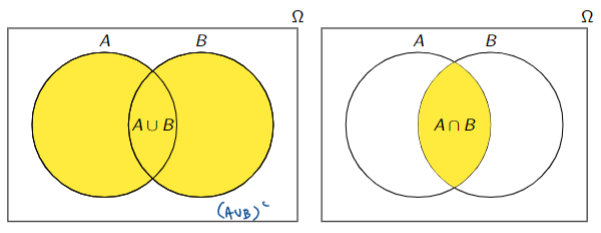
\includegraphics[scale=1]{2022-12-15-18-03-07.png}

        The definition of the intersection of events brings us to an important terminology of events:
        \dfn{Mutually Exclusive}{
            We say two events are \textbf{mutually exclusive} if $A\cap B=\emptyset$. Meaning the events can not occur simultaneously as an outcome of the random experiment. Synonymously denoted \textbf{disjoint} events.
        }
        The following laws of set relationships are useful when simplifying probabilities in the future:
        \begin{description}
            \item [Commutative Law]: $A \cup B = B \cup A$
            \item [Associative Law]: $ (A \cup B) \cup C = A \cup (B \cup C)$ \textit{(Same for intersection)}
            \item [Distributive Law]: $A \cap (B \cup C) = (A \cap B) \cup (A \cap C)$
            \item [DeMorgan's Laws of Union]: $(A\cup B)^C = A^C \cap B^C$
            \item [DeMorgan's Laws of Intersection]: $(A \cap B)^C = A^C \cup B^C$
        \end{description}


        \section{Introduction to Probability}
        Probability is a mathematical discipline that studies the likelihood of events occurring. It is used to model and analyze random phenomena, such as the roll of a dice or the outcome of a coin toss.
        Probability is defined as follows:

        \dfn{Probability}{
            For any random experiment with sample space $S$, and event $A\subseteq S$, the \textbf{probability} of event $A$ is denoted as $P(A)$. Where $P:S\rightarrow [0,1]$, is a function which assigns a value to an event. This value corresponds to the chance that an event A occurs
        }
        \vspace{.5cm}
         

        Probability theory is based on a set of axioms, or fundamental principles, that provide a consistent framework for calculating probabilities and making predictions. In this section, we will delve into the axioms of probability and their implications for the mathematical treatment of random events.

        The axioms of probability specify the rules for assigning probabilities to events. They are designed to capture the basic properties of probability, such as the fact that the probability of an event occurring must be a number between 0 and 1, inclusive. The axioms also provide a foundation for more advanced concepts in probability theory, such as conditional probability and independence. By studying the axioms of probability, we can gain a better understanding of the mathematical principles underlying the analysis of random events.

        \dfn{The Three Axioms of Probability}{
            \begin{enumerate}
                \item $P(A)\geq 0$
                \item $P(\Omega)= 1$
                \item For a set of disjoint events, $A_1, A_2, \dots, A_n$, in $\Omega$:
                \begin{equation*}
                    P\bigg ( \bigcup\limits_{i=1}^{n} A_i\bigg ) = \sum_{i=1}^{n}P(A_i)
                \end{equation*}
            \end{enumerate}
        }

        \ex{Using the Three Axioms in a Proof}{
            \begin{proof} $P(A) = 1 - P(A^C)$
                By the definition of compliment we have $A^C\cup A = \Omega$. Following this we get $P(A\cup A^C) = P(\Omega)$. Using the third axiom we can get that $P(A)+P(A^C) = P(\Omega) \rightarrow P(A) = P(\Omega) - P(A^C)$. Finally using the second axiom of probability we have that $P(A) = 1 - P(A^C)$.
            \end{proof}
        }

        \section{The Inclusion-Exclusion Principle} 

        when we are dealing with events that are not mutually exclusive, the basic principle of counting does not apply and we need a more sophisticated approach. This is where the inclusion-exclusion principle comes in.

The inclusion-exclusion principle is a powerful tool that allows us to calculate the probability of the union of two or more events in a precise and efficient way. It is based on the idea of "inclusion" and "exclusion" of elements, and it states that if we have a collection of events, then the probability of the union of these events is equal to the sum of the probabilities of the individual events, minus the probability of the intersection of any two events, plus the probability of the intersection of any three events, and so on. This alternating pattern of inclusion and exclusion allows us to account for the overcounting and undercounting of elements that occurs when we simply add up the probabilities of the individual events.

        \dfn{Inclusion-Exclusion Principle}{
            For any set of events, $A_1, A_2, \dots, A_n$, the probability of any of these events occuring is:
            \begin{align*}
                P\bigg ( \bigcup\limits_{i=1}^{n} A_i\bigg )
                =&\sum_{i=1}^{n}P(A_i) \\
                &- \sum_{i<j}P(A_i\cap A_j) \\
                &+ \dots \\
                & + (-1)^{r+1}\sum_{i_1<i_2<\dots<i_r}P(A_{i_1}\cap A_{i_2} \cap \dots \cap A_{i_r}) \\
                &+ \dots \\
                & + (-1)^{n+1}P(A_{i_1}\cap A_{i_2} \cap \dots \cap A_{i_n})
            \end{align*}
            
        }

        \ex{}{Suppose we have two events, $A$ and $B$, with probabilities $P(A) = 0.4$ and $P(B) = 0.6$. We want to find the probability of the union of these events, which we can denote as $P(A \cup B)$.

        Using the inclusion-exclusion principle, we can write:
        
        $$P(A \cup B) = P(A) + P(B) - P(A \cap B)$$
        
        To calculate the probability of the intersection of $A$ and $B$, $P(A \cap B)$, we need to know whether the events are mutually exclusive or not. If they are mutually exclusive, then $P(A \cap B) = 0$, and the probability of the union is simply the sum of the probabilities of the individual events:
        
        $$P(A \cup B) = P(A) + P(B) - P(A \cap B) = 0.4 + 0.6 - 0 = 1.0$$
        
        However, if the events are not mutually exclusive, then we need to know the probability of the intersection in order to calculate the probability of the union. For example, suppose $P(A \cap B) = 0.2$. Then the probability of the union is:
        
        $$P(A \cup B) = P(A) + P(B) - P(A \cap B) = 0.4 + 0.6 - 0.2 = 0.8$$
        
        This shows that the probability of the union of two events is equal to the sum of the probabilities of the individual events, minus the probability of the intersection of the events }


        \section{Probability as Relative Frequency}

        This final section prefaces counting and relates to the probability of some event occurring, given the probability of any outcome is equally likely to any other outcome. This can be summarized with the following

        \dfn{Probabiltiy as Relative Frequency}{
            If the probability of all outcomes in $\Omega$ are equal, then the probability of any event is the ratio of the size of the event to the size of $\Omega$. Formally described as:
            IF: $\forall e_1,e_2 \in \Omega. P(e_1)=P(e_2)$\\
            THEN: For all subsets of $\Omega$, $A$:
            \begin{equation*}
                P(A) = \frac{|A|}{|\Omega|}
            \end{equation*}
        }

        \nt{
            Relative Frequency can also mean the number of outcomes of $A$ being true given some number of trials. In this case the relative frequency of $A$ is the ratio of the number of occurences of $A$ and the number of trials.
        }


        \section{Conditional Probability}
        Considering different events allows us to have cases where two events occur. From the section on intersection, given two events, $A$ and $B$, they are considered to have ocurred at the same time if any outcome from $A\cap B$ has ocurred. Sometimes we want to consider the probability that an event has ocurred, given that we know that another event has ocurred. This concept may seem abstract; however, it is simplified by understanding the probability of an event occurring given we know another event ocurred by just imagining the probability of an event occurring given a new sample space. This new sample space is all the outcomes of the event we know occurred. This concept is called conditional probability.

        \dfn{Conditional Probability}{
            Let there be a random experiment with sample space $\Omega$. Let $A,B$ be events, $A\subseteq\Omega \wedge B\subseteq\Omega$, where $P(B)>0$. We denote the conditional probability of $A$ occuring given $B$ as:
            \begin{equation*}
                P(A|B)
            \end{equation*}
            We define \textbf{conditional probability} with the following:
            \begin{enumerate}
                \item $\forall b \in B. P(b|B)\geq 0$
                \item $\forall b_\omega\in\Omega-B. P(b_\omega|B)=0$
                \item $\sum_{b\in B}P(b|B)= 1$
                \item $P(A|B)=\sum_{a\in A}P(a|B)$
            \end{enumerate}
        }
        We can envision this concept as a venn diagram. The shade blue area is the sample space of the conditional probability, and the crossed area is the event $A|B$. $P(A|B)$ can be envisioned with:
        \begin{center}
            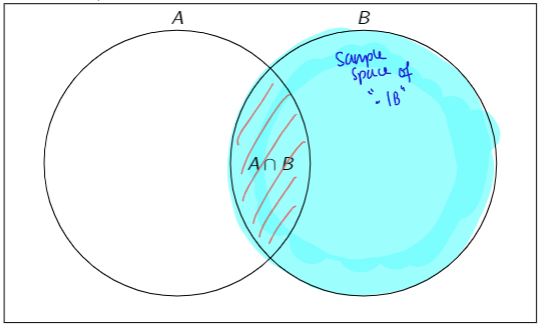
\includegraphics{2022-12-16-13-27-57.png}
        \end{center}

        \subsection{Closed Form of Conditional Probability}

        The definition of conditional probability lets us express it with the following:

        \begin{equation*}
            P(A|B) = \frac{P(A\cup B)}{P(B)}, \textnormal{where P(B)>0}
        \end{equation*}

        \subsection{Law of Total Probability}

        The law of total probability allows us to break down probabilities with conditional probabilities so that, sometimes, they are easier to work with. 

        \dfn{Law of Total Probability}{
            If $B_1, B_2, \dots, B_k$ is a collection of mutually exclusive and exhuastive partition of the sample space, then for any event $A$ we have:
            \begin{equation*}
                P(A)=\sum_{i=1}^{k}P(A|B_i)\cdot P(B_i)
            \end{equation*}
        }

        \section{Bayes' Rule}
        Using the Law of Total Probability with our definition of conditional probability we can expand and use Bayes' Rule:

        \dfn{Bayes' Rule}{
            Let $B_1, B_2, \dots, B_k$ form partition of the sample space. Let $A\subseteq \Omega$ be an event. Bayes' Rule states:
            \begin{equation*}
                P(B_i|A) = \frac{P(A|B_i)\cdot P(B_i)}{\sum_{i=1}^{k}P(A|B_i)\cdot P(B_i)}
            \end{equation*}
        }
        This rule is very abstract and initially confusing on how to use. However, it is very practical once understood.
        \ex{}{
            A ball is drawn at random from an urn containing one red and one
            white ball. If the white ball is drawn, it is put back into the urn. If the red ball is
            drawn, it is returned to the urn together with two more red balls. Then a second
            draw is made.\\
            First we will consider the probability that the red ball was drawn on both draws. We can represent this with two events, $R_1$ and $R_2$, the event that the red ball is drawn on the first draw and the event that the red ball is drawn on the second draw. We can represent our final probability as $P(R_1)\cdot P(R_2|R_1)=\frac{1}{2}+\frac{3}{4}=\frac{3}{8}$. This is easy to consider and we do not need to expand the definition of a conditional probability to understand it.\\\\
            Consider the probability of the first ball being chosen red given we know the second ball was red. This is represented as $P(R_1|R_2)$. We can understand this by expanding the definition and using Bayes' Rule:
            \begin{align*}
                P(R_1|R_2)&=\frac{P(R_1\cap R_2)}{P(R_2)}\\
                &=\frac{P(R_1\cap R_2)}{P(R_2|(\Omega-R_1))\cdot P(\Omega-R_1)+P(R_2|R_1)\cdot P(R_1)}\\
                &=\frac{\frac{3}{8}}{\frac{1}{4}+\frac{3}{8}}\\
                &= \frac{3}{5}
            \end{align*}
        }

        \section{Independent Events}
        The definition of the independence of an event can be defined and better understood using conditional probability. The informal definition of two events being independent is: given we know one event has occurred, the probability of the other occurring has not changed. Expressed with conditional probability:
        \dfn{Independent Events}{
            Let $A$ and $B$ be two events of some random experiment. $A$ and $B$ being independent is equiavalent to saying:
            \begin{equation*}
                P(A|B)=P(A)\wedge P(B|A)=P(B)
            \end{equation*}
            This assumes that $P(A)$ and $P(B)$ are both greater than $0$. An equivalent statement is:
            \begin{equation*}
                P(A\cap B)= P(A)\cdot P(B)
            \end{equation*}
            If $A$ and $B$ are not independent we consider them dependent.
        }

        This definition extends to multiple events. definition extends to another concept called mutual independence:
        \dfn{Independent Collection of Events}{
            For a collection of $n$ events, $A_1, A_2, \dots, A_n$, we consider they are independent if:
            $$P(A_1\cap \dots \cap A_n) = P()$$
        }
        \nt{
            We consider a collection events \textbf{mutually independent if any subset of the events are independent}
        }




    \chapter{Counting}
    Counting is a fundamental concept in probability, as it allows us to determine the number of possible outcomes in a given probability experiment. Understanding how to count the number of possible outcomes is essential for calculating the likelihood of different events occurring.

    Counting also plays a crucial role in understanding the relationships between different probability events. For example, knowing how to count the number of possible outcomes can help us understand how the probability of one event might be affected by the occurrence of another event.
    
    In addition to its practical applications, counting is also a fundamental mathematical concept that is closely related to other areas of mathematics, such as combinatorics and graph theory. As such, a strong understanding of counting principles is important for anyone interested in pursuing a career in mathematics or a related field.

    \section{Fundamental Principle of Counting}

    When applying probability as a relative frequency it is important to be able to understand the number of possible outcomes in some experiment. Often we represent experiments as more complicated versions of others. One way we compliment experiments is adding stages. Meaning that we repeat the same experiment, or others, multiple times and record the combined outcome of every stage.

    \dfn{Fundamental Principle of Counting}{
        If an experiment consists of $m$ (ordered) stages with $n_2$ possible outcomes in
        stage 1, $n_2$ possible outcomes in stage 2, $\dots$, $n_m$ possible outcomes in stage $m$,
        then the total number of possible outcomes is:
        \begin{equation*}
            \prod_{i=1}^{m}n_i=n_1\cdot n_2\cdot\dots\cdot n_m
        \end{equation*}
    }

    

    \ex{}{
        $\text{If there are }m\text{ ways to perform task 1 and }n\text{ ways to perform task 2, then there are }$ $m \times n$\\ $ \text{ ways to perform both tasks.}$

This principle is often used in combinatorics and probability to determine the number of possible outcomes in a given situation. For example, if you have 3 choices for one task and 4 choices for another task, then there are $3 \times 4 = 12$ possible combinations of the two tasks.
    }

    \nt{
        The Fundamental Principle of Counting is specific to ordered stages. This means we know the order of sub-experiments we will use. To understand when the stages are not ordered we must first understand permutations and combinations.
    }

    \section{Permutations}

    When counting the number of possible ways unordered stages can occur we have to consider all the possibilities by understanding all the different ways to order the stages in terms of the number of possible stages $n$, and, optionally, the number of stages we must consider, $k$.

    \dfn{Permutation - $_nP_k$}{
        The number of ways to select an ordered subset of $k$ items from a group of $n$ distinct items is:
        \begin{equation*}
            _{n}P_{k}=\frac{n!}{(n-k)!}
        \end{equation*}
    }

    \ex{}{
        Suppose we have a bag containing 3 balls: red, green, and blue. If we draw 3 balls from the bag without replacement (meaning that we don't put the balls back in the bag after drawing them), the possible outcomes of the order of the balls are the permutations of the 3 balls. Using the formula above, we can calculate the number of permutations as follows:

$$P_3 = 3! = 3 \times 2 \times 1 = 6$$

Therefore, there are 6 possible outcomes for this experiment: red-green-blue, red-blue-green, green-red-blue, green-blue-red, blue-red-green, and blue-green-red.
    }

    \section{Indistinguishable Objects}

    Some times we are trying to track the permutation of some objects, however we must be careful to not count duplicate permutations where only duplicate objects have been rearranged.

    \ex{Indistinguishable Objects}{
        An urn contains 4 red balls, 1 yellow ball, 3 green balls, and 2 blue balls. How many different ways are there to arrange all 10 of these balls?
    }

    This problem may seem simple. All we must do is find the permutation of 10 distinct objects, $_{10}P_{10}$. However, the issue is that these objects are not actual distinct. If we calculated the total number of outcomes this way we would end up with the following duplicate ordering:
    \begin{center}
        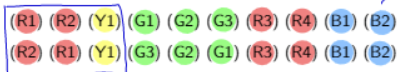
\includegraphics{2022-12-16-12-30-26.png}    
    \end{center}
    To fix this we can try and consider every possible way each ordering of indistinct objects can repeat, and then divide our incorrect permutation with that. In this case there are $4$ red balls, and hence $4!$ ways to order them. Combining this for each set of colored balls we get that there are $4!3!1!2!=288$ ways to order every permutation we counted earlier. Therefore we divide the previous answer to get $\frac{10!}{288}=12600$ ways to order the 10 balls.


    \section{Combinations}

    Permutations describe an experiment where the stages, or objects, and the order of the stages, or objects we are tracking, is unclear. On the other hand there are cases when in a random experiment we known the order of the objects, or do not care, yet the possible objects are unclear.
    \ex{}{
        Consider the 5 letters, ABCDE and we want to select only three (unordered)
        letters. This means the selection ABC includes selections of BAC. How many
        unique groups of 3 letters are possible?\\\\
        In this example it is obvious that this encompasses some sort of permutation of the letters, as we randomly select three. However, the issue is that calculating $_{5}P_{3}$ includes duplicates such as $ABC$ and $CBA$. These two examples may seem different, but in the domain of our question, which ignores order, these instances are considered the same outcome. Instead we need to consider, just like for when calculating Indistinguishable objects, the number of duplicate permutations for every single permutation. For this we have to consider the number of ways to order the $3$ letters. There are $3!$ ways to order three elements. This means that every permutation has $3!$ duplicates. So to find the answer we have to calculate:
         $$\frac{_{5}P_{3}}{3!}$$.
    }

    From this example we had to find the number of combinations of $3$ elements where there are $5$ to choose from. Unsurprisingly, this concept of counting is called, combinations. 

    \dfn{Combinations - $_{n}C_{k}$}{
        The number of ways to select an \textit{unordered} subset of $k$ items from a group of $n$ \textbf{distinct} items without replacement is:
        \begin{equation*}
            \binom{n}{k}=_{n}C_{k}=\frac{n!}{(n-k)!k!}
        \end{equation*}
    }

    \nt{
        The formula for combinations is derived from the formula for permutations. The extra $k!$ has to do with there being $k!$ ways to order every single combination. 
    }



    



    \chapter{Random Variables}

    A random variable is a function that assigns a numerical value to each outcome of a random experiment. It is a way to represent the outcomes of a random process or experiment in a numerical form.

    Random variables are an important concept in probability and statistics because they allow us to describe and analyze random processes and experiments. By assigning numerical values to the outcomes of a random experiment, we can use tools from mathematics and statistics to analyze the behavior and characteristics of the random process.

    There are two main types of random variables: discrete and continuous. A discrete random variable is one that can take on only a finite or countably infinite number of values, such as the number of heads obtained when flipping a coin three times. A continuous random variable is one that can take on any value within a given range, such as the height of a person.

    Understanding and working with random variables is a crucial skill for anyone interested in data analysis, statistical modeling, and other fields that involve the analysis of random processes and experiments.

    \section{Introduction to Random Variables}

    \dfn{Random Variable}{
        A \textbf{random variable} is a real-valued function that assigns a numerical value to each event in the sample space $\Omega$ arising from a random experiment. A random variable $X$ is a real-valued function $X :\Omega \rightarrow \bbR $ such that for every $\omega \in \Omega. X(\omega) = x \in \bbR$. It is a mapping from the sample space to the real numbers, representing the outcome.
    }

    \ex{Using Random Variables}{
        Consider the experiment of tossing a coin with sample space $\Omega = \{H, T\}$
        Let $X$ be the outcome of a toss. We can define $X$ such that when $X=1$ corresponds to $H$ and when $X=0$ corresponds to $T$.
    }

    \nt{
        The convention for random variables is to express them with capital letters and when interpretting their unknown value we use the lower case version. An example being for some random variable $X$ we consider its possible probabilities as $P(X=x)$.
    }


    \section{PMF of Discrete Random Variables}
    A discrete of a random variable X is one that can take on only a finite number or a countably infinite number of possible values x. The probability mass function of a discrete random variables assigns a probability to each value $x\in X$, such that we can understand the probability of that value occurring.
    \dfn{Probability Mass Function of a Discrete Random Variable}{
        Let $X$ be a random variable. The \textbf{probability mass function} of $X$ is such that for every $x \in X$ we assign a probability where:
        \begin{enumerate}
            \item $0\leq P(X=x) \leq 1$
            \item $\sum_{x\in X}P(X=x) = 1$
        \end{enumerate}
    }
    \ex{Finding a PMF}{
        A factory producing computer parts sends out a shipment of 10 parts of
    which 3 are defective. Find the probability mass function for the number of
    defectives a customer will get if the first customer randomly purchases 4
    computer parts.\\
    For this question we have to quantify the probability of each possible number of defective parts the customer recieves. We know that this value will be between $0-3$ as the customer buys $4$ parts. We can think of this quesiton as various combinations of parts, good and bad. Let $D$ be the number of defective parts:
    \begin{align*}
        P(D=0) &= \frac{\binom{7}{4}}{\binom{10}{4}}\\
        P(D=1) &= \frac{\binom{7}{3}\binom{3}{1}}{\binom{10}{4}}\\
        P(D=2) &= \frac{\binom{7}{2}\binom{3}{2}}{\binom{10}{4}}\\
        P(D=3) &= \frac{\binom{7}{1}\binom{3}{3}}{\binom{10}{4}}\\
        P(D=d) &= \frac{\binom{7}{4-d}\binom{3}{d}}{\binom{10}{4}}
    \end{align*}
    }

    \nt{
        Discrete Distributions and their probability mass functions can be thought of as histograms/bar charts. This is expanded on in the Discrete PRobability Distributions chapter.
    }

    \section{Characteristics of Random Variables}
    \subsection{Expected Values}
    The expected value lets us track the mean of Random Variables:
    \dfn{Expected Value}{
        The long run/theoretical average. If a random experiment
        were to be conducted $n$ times, then as $n\rightarrow\infty$then the average of outcomes converges to the expected value. This is often denoted as $\mu$. For any random variable $X$, its expected value is denoted and defined as:
        \begin{equation*}
            E[X]=\mu=\sum_{x\in X}x\cdot P(X=x)
        \end{equation*}
        For any transformation of $X$, $g(X)$, we define the expected value of this transformation of $X$ similarly:
        \begin{equation*}
            E[g(X)]=\sum_{x\in X}g(x)\cdot P(X=x)
        \end{equation*}

    }
    \nt{
        $E[g(X)]\neq g(E[X])$ unless $g(X)$ is only a linear transformation.
    }

    \subsection{Variance}
    The variance of a random experiment or random variable expressed the spread and variability of results:
    \dfn{Variance \& Standard Deviation}{
        The \textbf{variance} of $X$ is defined to be
        \begin{equation*}
            \sigma^{2}=V(X) = E[(x-\mu)^{2}] = \sum_{x\in X}(x-\mu)^2\cdot P(X=x)
        \end{equation*}
        Variance captures the spread in \textit{units}$^2$. The standard deviation, $\sigma=\sqrt[]{\textnormal{variance}}$ is the average spread, or distance from the mean, the random variable is.
    }

    \subsection{Properties of Expectation and Variance}

    For any constants, $a$ and $b$, and discrete random variables, $X$ and $Y$, the following properties of expectation is true: \vspace{.5cm}
     
    \cor{Properties of Expectation}{
        \begin{enumerate}
            \item $E[a]=a$
            \item $E[X+a]=E[X+a]$
            \item $E[aX]=a\cdot E[X]$
            \item $E[aX+b]= a \cdot E[X]+ b$
            \item $E[X+Y]=E[X]+E[Y]$
            \item If $X$ and $Y$ are independent: $E[XY]=E[X]\cdot E[Y]$
        \end{enumerate}
    }
    \vspace{.5cm}
     
    For any constants, $a$ and $b$, and discrete random variables, $X$ and $Y$, the following properties of variance is true: \vspace{.5cm}
    \cor{}{
        \begin{enumerate}
            \item $V(a)=0$
            \item $V(a+X)=V(X)=\sigma^{2}$
            \item $V(aX)=a^{2}\cdot V(X)=a^{2}\cdot \sigma^{2}= a^2E[(X-\mu)^{2}]$
            \item $V(aX+b)=a^2\cdot V(X)=a^2\cdot\sigma^{2}$
            \item IF X and Y are independent $V(X+Y)=V(X+)V(Y)$
        \end{enumerate}
    }

    \section{Cumulative Distribution Function}
    \dfn{}{
        The cumulative distribution function (CDF) F (x ) of a discrete random variable
        with probability mass function P (x ) or f (x ) is a function that returns the
        cumulative (total) probability up to and including X = x.
        \begin{equation*}
            F(b)=P(X\leq b)= \sum_{x\in\{ x\leq b\}}P(x)
        \end{equation*}
The domain of the CDF is always over the set of real numbers! As such, CDFs
are often represented as a piecewise function.
    }


    




    \chapter{Discrete Probability Distributions}





    \chapter{Continuous Probability Distributions}





    \chapter{Multivariate Distributions}





    \chapter{Central Limit Theorem}



    

\end{document}